\documentclass[bigger]{beamer}
\usepackage[utf8]{inputenc}
\usepackage{graphicx}
\usepackage{pgfplots}
\usepackage{tabularx}

\setbeamertemplate{navigation symbols}{}%remove navigation symbols
\setbeamertemplate{caption}{\raggedright\insertcaption\par}

\begin{document}

\begin{frame}
  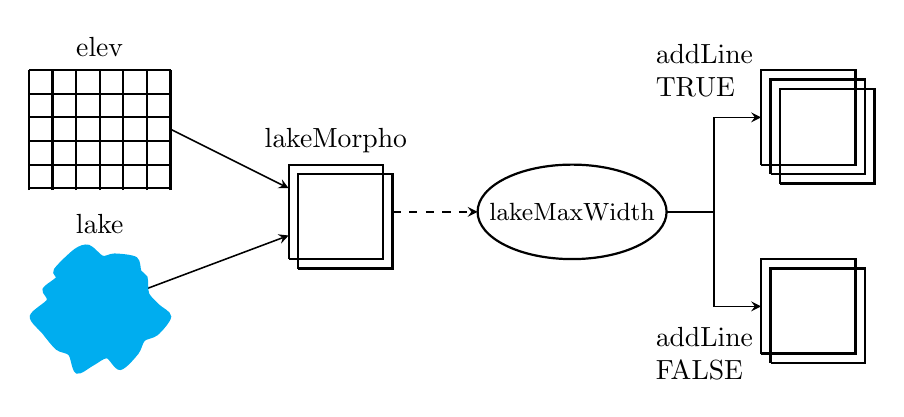
\begin{tikzpicture}[scale = 0.6]
    \draw[>=stealth, ->, line width = 0.2mm] (0, 0) -- (4, 1.5);
    \draw[cyan, ultra thick, domain=0:350, smooth cycle, fill=cyan] 
        plot (\x:1+rnd*0.5);
    \node at (0, 1.75) {lake};
    
    \draw[>=stealth, ->, line width = 0.2mm] (1.5, 3.75) -- (4, 2.5);
    \draw[step=0.5, thick] (-1.5, 2.46) grid (1.5, 5);
    \node at (0, 5.5) {elev};
    
    \draw[thick] (4,1) -- (6,1) -- (6,3) -- (4,3) -- (4,1);
    \draw[thick] (4.2,0.8) -- (6.2,0.8) -- (6.2,2.8) -- (4.2,2.8) -- (4.2,0.8);
    \node at (5, 3.5) {lakeMorpho};
    
    \draw[>=stealth, ->, line width = 0.2mm, dashed] (6.2, 2) -- (8, 2);
    \draw[thick] (10, 2) ellipse (2cm and 1cm);
    \node at (10, 2) {\small lakeMaxWidth};
    
    \draw[>=stealth, ->, line width = 0.2mm] (12, 2) -- (13,2)-- (13, 4) -- (14, 4);
    \node[align = left] at (12.8, 5) {addLine \\  TRUE};
    
    \draw[>=stealth, ->, line width = 0.2mm] (12, 2) -- (13,2) -- (13, 0) -- (14, 0);
    \node[align = left] at (12.8, -1) {addLine \\  FALSE};
    
    \draw[thick] (14,3) -- (16,3) -- (16,5) -- (14,5) -- (14,3);
    \draw[thick] (14.2,2.8) -- (16.2,2.8) -- (16.2,4.8) -- (14.2,4.8) -- (14.2,2.8);
    \draw[thick] (14.4,2.6) -- (16.4,2.6) -- (16.4,4.6) -- (14.4,4.6) -- (14.4,2.6);
    
    \draw[thick] (14,-1) -- (16,-1) -- (16,1) -- (14,1) -- (14,-1);
    \draw[thick] (14.2,-1.2) -- (16.2,-1.2) -- (16.2,0.8) -- (14.2,0.8) -- (14.2,-1.2);
    
  \end{tikzpicture}

\end{frame}

\end{document}
